\documentclass{article}
\usepackage{blindtext}
\usepackage{authblk}
\usepackage[utf8]{inputenc}
\usepackage{amsmath, amssymb}
\usepackage{amssymb}
\usepackage[overload]{empheq}
\usepackage[font=small,labelfont=bf]{caption}
\usepackage{subcaption}
\usepackage{hyperref}
 % Required for specifying captions to tables and figures

\newcommand{\for}{\text{for }}
 
\title{SPM project: Parallel Prefix}
\author{Gaspare Ferraro, 520549}
\affil{Master Degree in Computer Science - University of Pisa}
\affil[]{ferraro@gaspa.re}
\date{\today}
 
\begin{document}
 
\maketitle
 
%%%%%%%%%%%%%%%%%%%%%%%%%%%%%%%%%%%%%%%%%%%%%%%%%%%%%%%%%%%%%%%%%%%%%%%%%%%%%%%
\section{Introduction}

In this report we will analyze, theoretically and practically, the resolution of the problem of the (parallel) prefix sum:

\medskip

\textit{Given a vector $x = \langle x_{0}, x_{1}, \ldots, x_{n-1} \rangle$ and a binary operation $\oplus$ compute the vector $y = \langle x_{0}, x_{0} \oplus x_{1}, x_{0} \oplus x_{1} \oplus x_{2}, \ldots, x_{0} \oplus x_{1} \oplus \ldots \oplus x_{n-1} \rangle$.} % , i.e. each element of the output vector at position $i$ is the results of 

\medskip

In literature this operation is also called (inclusive) scan or partial sum.

\medskip

For the analysis of the problem we have to make two assumptions:

\begin{itemize}
  \item The binary operation $\oplus$ is associative ($ a \oplus ( b \oplus c ) =  (a \oplus b) \oplus c  $) and commutative ($a \oplus b = b \oplus a$), this is an important assumption as we will see in the next chapters the order of the operations may not be preserved.
  \item The size of the input vector is a power of $2$, not a strong assumption, as all the algorithms we will present could be easily generalize to all the sizes, but it only helps to simplify some operations.
\end{itemize}

%%%%%%%%%%%%%%%%%%%%%%%%%%%%%%%%%%%%%%%%%%%%%%%%%%%%%%%%%%%%%%%%%%%%%%%%%%%%%%%
\section{Sequential algorithm}

The sequential algorithm simple compute each element of the vector $y$ as follow:

\begin{equation*}[]
    y_{i} =
    \begin{cases}
      x_{0}& \for i = 0 \\
      x_{i} \oplus y_{i-1},& \for 0 <  i < n
    \end{cases}
\end{equation*}

This algorithm is optimal in a sequential model as it has a running time of $\mathcal{O}(n)$, assuming that $\oplus$ is $\mathcal{O}(1)$, and performs $n-1$ calls to $\oplus$ operation.
 
%%%%%%%%%%%%%%%%%%%%%%%%%%%%%%%%%%%%%%%%%%%%%%%%%%%%%%%%%%%%%%%%%%%%%%%%%%%%%%%
\section{Parallel architecture design}

The problem of computing the prefix sum vector is a classical example of a problem that have an optimal solution in a sequential model but that can be optimized in a parallel model. 
The optimization is not in terms of total complexity or in the number of $\oplus$ operations performed (which are already optimals in the sequential algorithm) but in terms of completion time. When the number of available workers is more than one we can trade-off more total work for less completion time.
\medskip

We will now introduce two different algorithms that solve in an efficient way the prefix sum problem in a parallel model. 

\subsection{Block-based algorithm}

The idea behind the first parallel algorithm is to compute the prefix vector in three phases:

\begin{itemize}
  \item Partitionate the input vector in blocks and compute in parallel the prefix vector of each of them.
  \item In the second phase we put the final element of each block in a temporary vector and compute its prefix vector.
  \item Finally for each block $i$ (except for the first one) add in parallel the $(i-1)$th element of the temporary vector.
\end{itemize}

At the end of the three phases the final vector contains the correct prefixes.

\begin{center}
\begin{minipage}{0.65\linewidth}
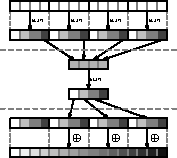
\includegraphics[width=\linewidth]{img/block}
\captionof{figure}{Block-based algorithm graphic representation} 
\end{minipage}
\end{center}

\subsection{Circuit-based algorithm}

Another class of algorithms are the one based on a circuit-like representation. A generic prefix circuit $C$ is a collection of tasks $T_1, T_2, \ldots, T_t,$ . 
A task $T_i$ is a set of operations $(l, r)$ that means to compute $x_r = x_r \oplus x_l$. The tasks must be computed sequentially from $1$ to $t$ but the advantage is that all the operations in a same task can be performed in parallel without race conditions.

\medskip

For example the sequential algorithm seen before can be represented as a prefix circuit $S(n) = \{ T_{1}, T_{2}, \ldots, T_{n-1} \}$ where $T_{i} = \{ (i-1, i) \}$.

\medskip

We present now the simple (but still efficient) prefix circuit $P(2^m)$:

\begin{equation*}
  P(2^m) = \{ T_1, T_2, \ldots, T_m, T_{m+1}, \ldots, T_{2m-1} \}  
\end{equation*}
where $\text{for}\ i = 1, \ldots, m$:
\begin{equation*}
  T_i = \{ (2k^i - 2^{i-1}-1, 2k^i-1 )\ |\ k = 1, \ldots, 2^{m-i} \}
\end{equation*}
and $\text{for}\ i = 1, \ldots, m-1$:
\begin{equation*}
  T_{m+i} = \{ (k2^{m-i}-1, k2^{m-i}+2^{m-i-1}-1 )\ |\ k = 1, \ldots, 2^{i}-1 \}\
\end{equation*}

\medskip

In the first phase (from $1$ to $m$) we compute operations like in a reduction tree, in the second phase (from $m+1$ to $2m -1$) we compute the final value of each prefix as the sum of only two others values.

\begin{figure}[h]
\centering
\begin{subfigure}{.5\textwidth}
  \centering
  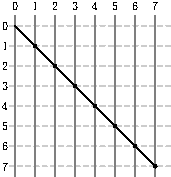
\includegraphics[width=.9\linewidth]{img/circuit-serial}
  \caption{Prefix circuit $S(8)$}
  \label{fig:sub1}
\end{subfigure}%
\begin{subfigure}{.5\textwidth}
  \centering
  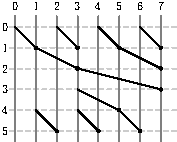
\includegraphics[width=.9\linewidth]{img/circuit-parallel}
  \caption{Prefix circuit $P(8)$}
  \label{fig:sub2}
\end{subfigure}
\caption{Examples of prefix circuits}
\label{fig:test}
\end{figure}

As we can see in these simple examples, for $n = 8$ the sequential algorithm needs $7$ units of time against the only $5$ of the parallel algorithm (obviously if the number of workers is at least $4$). 

%%%%%%%%%%%%%%%%%%%%%%%%%%%%%%%%%%%%%%%%%%%%%%%%%%%%%%%%%%%%%%%%%%%%%%%%%%%%%%%
\section{Performance modeling}

For the theoretical performance modeling we will denote with:

\begin{itemize}
  \item $n = 2^m$ the size of the input vector ($m = \log_2{n}$).
  \item $p$ the parallelism degree (for simplicity $p \leq n$).
  \item $t_{\oplus}$ is the time to compute a single $\oplus$ operation.
\end{itemize} 

\subsection{Sequential algorithm}

The completion time of the sequential algorithm is simply $T^{s}_C = (n-1) \times t_{\oplus}$. 

\subsection{Block-based algorithm}

The parallel completion time of the block-based algorithm is the sum of the completion times of all of the three phases:

\begin{equation*}
  T^{b}_{C_p} \geq T_{1_p} + T_{2_p} + T_{3_p}
\end{equation*} 

Where:

\begin{itemize}
  \item $T_{1_p} = (n/p) \times t_{\oplus}$ is the time to compute the prefix sums of a single block (as all the $p$ blocks are performed in parallel).
  \item $T_{2_p} = p \times t_{\oplus}$ is the time to compute the prefix sums over the temporary vector.
  \item $T_{3_p} = (n/p) \times t_{\oplus}$ (or $0$ if $p = 1$) is the time to add a value to a single block (except the first one).
\end{itemize}

So the total completion time is $T^{b}_{C_p} \geq (2n/p + p) \times t_{\oplus}$.

\smallskip

In this analysis we assume that $n$ is a multiple of $p$ and all the blocks have the same size, if this is not the case we can consider the block size as the size of the biggest block.

\subsection{Circuit-based algorithm}

In the prefix circuit $P(n)$ we have a total of $2m-1$ tasks that must be executed sequentially. 
As said before all the operations in the same task can be performed in parallel at the same time, so a generic task $T_i$ has a completion time of $1 \times t_{\oplus}$.

So the completion time of the algorithm is $T^{c}_{C_p} \geq (2\log_{2}(n) - 1) \times t_{\oplus}$.

\smallskip

However this analysis works only if the parallelism degree is high enough to allow to performs all the operations in $T_i$ at the same time ($p \geq n/2$).

\smallskip

When this is not the case a task $T_i$ is perfomed in $\max(1, |T_i|/p) \times t_\oplus$ time and the completion time is circa $T^{c}_{C_p} \simeq 2(\log_2{p} + n/p) \times t_{\oplus}$.

\subsection{Comparison table}

Now we can compare the completion time of all the algorithms:

\begin{table}[h]
\centering
\begin{tabular}{|c|r|r|r|}
\hline
 $p$ & $T^s_{C}$                & $T^b_{C_p}$                   & $T^c_{C_p}$ \\ \hline
  1  & $(n-1)\times t_{\oplus}$ & $n \times t_{\oplus}$         & $2n \times t_{\oplus}$\\ \hline
  2  & $(n-1)\times t_{\oplus}$ & $n \times t_{\oplus}$         & $(n+2) \times t_{\oplus}$ \\ \hline
  4  & $(n-1)\times t_{\oplus}$ & $(n/2 + 4) \times t_{\oplus}$ & $(n/2+4) \times t_{\oplus}$ \\ \hline
  8  & $(n-1)\times t_{\oplus}$ & $(n/4 + 8) \times t_{\oplus}$ & $(n/4+3) \times t_{\oplus}$ \\ \hline
 ... & ...                      & ...                           & ... \\ \hline
 n/2 & $(n-1)\times t_{\oplus}$ & $(n/2+1)\times t_{\oplus}$    & $2(\log_{2}(n) + 1) \times t_{\oplus}$ \\ \hline
  n  & $(n-1)\times t_{\oplus}$ & $(n+2)\times t_{\oplus}$      & $2(\log_{2}(n) + 1) \times t_{\oplus}$ \\ \hline
\end{tabular}
\caption{Comparison of the three algorithms with different parallelism degrees}
\end{table}

What we can see from the table is that until $p = 2$ the improvement is negligible, but when the parallelism degree increase the parallel algorithms .

The circuit-based algorithm reach its best performance for $p \geq n/2$ where each task is computed in $1 \times t_{\oplus}$. 
The block-based algorithm scale as well as the circuit-based, but when the parallelism degree increase we have a lack of performance due the trade-off between the parallel part of the first and the third stage ($2n/p \times t_{\oplus}$) and the second stage that must be performed sequentially ($p \times t_{\oplus}$).

%induced for the second phase of the algorithm as it does a serial computation of $p \times t_{\oplus}$.

%%%%%%%%%%%%%%%%%%%%%%%%%%%%%%%%%%%%%%%%%%%%%%%%%%%%%%%%%%%%%%%%%%%%%%%%%%%%%%%
\section{Implementations structure and details}

All the implementations are written in C++17, the source code is available as attachment with the report or on \href{https://github.com/GaspareG/ParallelPrefix}{GitHub}.

Both of the parallel algorithms have been implemented using the standard C++ threads, the FastFlow framework and the OpenMP/Cilk Plus API. All the algorithms are designed to avoid race conditions between the operations in the same phase, so there is no need for any special synchronization mechanism except for the barriers at the end of each phase to pass to the next one.

Each different implementation is available as single class in a single \textit{.hpp} file. All the classes provide the methods to change the parallelism degree, to start the computation and to get time statistics of last computation.

\smallskip

Among with the implementions the project include a benchmark suite that provide different features for the tests: select which algorithm execute, select the range of input size, select the range for the parallelism degree and many other options.

\smallskip

To compile the project is enough to run the \textit{compile.sh} script inside the project folder.
If needed a short help is available for consultation, just run \textit{./benchmark -h}.

\subsection{Sequential algorithm}

The sequential implementations is simply an iteration over the input vector likely the implementation of the \textit{std::partial\_sum} function.

\subsection{Block-based algorithm}

TODO

\subsection{Circuit-based algorithm}

TODO

%%%%%%%%%%%%%%%%%%%%%%%%%%%%%%%%%%%%%%%%%%%%%%%%%%%%%%%%%%%%%%%%%%%%%%%%%%%%%%%
\section{Experimental validation}

The experiments were executed on a CPU \textit{Xeon Phi KNC} with $64$ physical core, each of them with a four-way multithreading support (for a total of $256$ threads).

\begin{itemize}
  \item Each running time is expressed in milliseconds and it is an average of $5$ repeated test.
  \item Each implemented algorithm was tested with $p \in \{1, 2, 4, 8, 16, 32, 64, 128\}$.
  \item Each implemented algorithm was tested with $n \in \{2^{20}, 2^{21}, \ldots, 2^{28}, 2^{29}\}$.
\end{itemize}

TODO


\subsection{experiments details}

TODO

\subsection{benchmark results}

TODO

%%%%%%%%%%%%%%%%%%%%%%%%%%%%%%%%%%%%%%%%%%%%%%%%%%%%%%%%%%%%%%%%%%%%%%%%%%%%%%%
\section{Conclusion}

TODO

%%%%%%%%%%%%%%%%%%%%%%%%%%%%%%%%%%%%%%%%%%%%%%%%%%%%%%%%%%%%%%%%%%%%%%%%%%%%%%%
\end{document}
